
%%%%%%%%%%%%%%%%%%%%%%%%%%%%%%%%%%%%%%%%%%%%%%%%%%%%%%%%%%%%%%%%%%%%%
%% This is a (brief) model paper using the achemso class
%% The document class accepts keyval options, which should include
%% the target journal and optionally the manuscript type.
%%%%%%%%%%%%%%%%%%%%%%%%%%%%%%%%%%%%%%%%%%%%%%%%%%%%%%%%%%%%%%%%%%%%%
\documentclass[journal=acsnano,manuscript=article]{achemso}

%%%%%%%%%%%%%%%%%%%%%%%%%%%%%%%%%%%%%%%%%%%%%%%%%%%%%%%%%%%%%%%%%%%%%
%% Place any additional packages needed here.  Only include packages
%% which are essential, to avoid problems later. Do NOT use any
%% packages which require e-TeX (for example etoolbox): the e-TeX
%% extensions are not currently available on the ACS conversion
%% servers.
%%%%%%%%%%%%%%%%%%%%%%%%%%%%%%%%%%%%%%%%%%%%%%%%%%%%%%%%%%%%%%%%%%%%%
\usepackage[version=3]{mhchem} % Formula subscripts using \ce{}
\usepackage[T1]{fontenc}       % Use modern font encodings
\usepackage{graphicx}
\usepackage{subcaption}
\usepackage{fixltx2e}
\usepackage{color}

%%%%%%%%%%%%%%%%%%%%%%%%%%%%%%%%%%%%%%%%%%%%%%%%%%%%%%%%%%%%%%%%%%%%%
%% If issues arise when submitting your manuscript, you may want to
%% un-comment the next line.  This provides information on the
%% version of every file you have used.
%%%%%%%%%%%%%%%%%%%%%%%%%%%%%%%%%%%%%%%%%%%%%%%%%%%%%%%%%%%%%%%%%%%%%
%%\listfiles

%%%%%%%%%%%%%%%%%%%%%%%%%%%%%%%%%%%%%%%%%%%%%%%%%%%%%%%%%%%%%%%%%%%%%
%% Place any additional macros here.  Please use \newcommand* where
%% possible, and avoid layout-changing macros (which are not used
%% when typesetting).
%%%%%%%%%%%%%%%%%%%%%%%%%%%%%%%%%%%%%%%%%%%%%%%%%%%%%%%%%%%%%%%%%%%%%
\newcommand*\mycommand[1]{\texttt{\emph{#1}}}
\newcommand\crule[3][black]{\textcolor{#1}{\rule{#2}{#3}}}
\newcommand{\angstrom}{\textup{\AA}}
\graphicspath{{snapshots/},{benzene/},{hphilic/}}

%%%%%%%%%%%%%%%%%%%%%%%%%%%%%%%%%%%%%%%%%%%%%%%%%%%%%%%%%%%%%%%%%%%%%
%% Meta-data block
%% ---------------
%% Each author should be given as a separate \author command.
%%
%% Corresponding authors should have an e-mail given after the author
%% name as an \email command. Phone and fax numbers can be given
%% using \phone and \fax, respectively; this information is optional.
%%
%% The affiliation of authors is given after the authors; each
%% \affiliation command applies to all preceding authors not already
%% assigned an affiliation.
%%
%% The affiliation takes an option argument for the short name.  This
%% will typically be something like "University of Somewhere".
%%
%% The \altaffiliation macro should be used for new address, etc.
%% On the other hand, \alsoaffiliation is used on a per author basis
%% when authors are associated with multiple institutions.
%%%%%%%%%%%%%%%%%%%%%%%%%%%%%%%%%%%%%%%%%%%%%%%%%%%%%%%%%%%%%%%%%%%%%
\author{Lisa E. Felberg}
\affiliation{Department of Chemical and Biomolecular Engineering, University of California Berkeley, Berkeley, California 94720, USA}
\author{Luis A. Ruiz Pestana}
\affiliation{Chemical Sciences Division, Lawrence Berkeley National Labs, Berkeley, California 94720, USA}
\author{Teresa Head-Gordon}
\affiliation{Department of Chemical and Biomolecular Engineering, University of California Berkeley, Berkeley, California 94720, USA}
\alsoaffiliation{Chemical Sciences Division, Lawrence Berkeley National Labs, Berkeley, California 94720, USA}
\alsoaffiliation{Department of Chemistry, University of California Berkeley, Berkeley, California 94720, USA}
\alsoaffiliation{Department of Bioengineering, University of California Berkeley, Berkeley, California 94720, USA}
\email{thg@berkeley.edu}

%%%%%%%%%%%%%%%%%%%%%%%%%%%%%%%%%%%%%%%%%%%%%%%%%%%%%%%%%%%%%%%%%%%%%
%% The document title should be given as usual. Some journals require
%% a running title from the author: this should be supplied as an
%% optional argument to \title.
%%%%%%%%%%%%%%%%%%%%%%%%%%%%%%%%%%%%%%%%%%%%%%%%%%%%%%%%%%%%%%%%%%%%%
\title[confinement]
  {Confinement}

%%%%%%%%%%%%%%%%%%%%%%%%%%%%%%%%%%%%%%%%%%%%%%%%%%%%%%%%%%%%%%%%%%%%%
%% Some journals require a list of abbreviations or keywords to be
%% supplied. These should be set up here, and will be printed after
%% the title and author information, if needed.
%%%%%%%%%%%%%%%%%%%%%%%%%%%%%%%%%%%%%%%%%%%%%%%%%%%%%%%%%%%%%%%%%%%%%
\abbreviations{IR,NMR,UV}
\keywords{confinement, 2D water}

%%%%%%%%%%%%%%%%%%%%%%%%%%%%%%%%%%%%%%%%%%%%%%%%%%%%%%%%%%%%%%%%%%%%%
%% The manuscript does not need to include \maketitle, which is
%% executed automatically.
%%%%%%%%%%%%%%%%%%%%%%%%%%%%%%%%%%%%%%%%%%%%%%%%%%%%%%%%%%%%%%%%%%%%%
\begin{document}

%%%%%%%%%%%%%%%%%%%%%%%%%%%%%%%%%%%%%%%%%%%%%%%%%%%%%%%%%%%%%%%%%%%%%
%% The "tocentry" environment can be used to create an entry for the
%% graphical table of contents. It is given here as some journals
%% require that it is printed as part of the abstract page. It will
%% be automatically moved as appropriate.
%%%%%%%%%%%%%%%%%%%%%%%%%%%%%%%%%%%%%%%%%%%%%%%%%%%%%%%%%%%%%%%%%%%%%
\begin{tocentry}

Some journals require a graphical entry for the Table of Contents.
This should be laid out ``print ready'' so that the sizing of the
text is correct.

Inside the \texttt{tocentry} environment, the font used is Helvetica
8\,pt, as required by \emph{Journal of the American Chemical
Society}.

The surrounding frame is 9\,cm by 3.5\,cm, which is the maximum
permitted for  \emph{Journal of the American Chemical Society}
graphical table of content entries. The box will not resize if the
content is too big: instead it will overflow the edge of the box.

This box and the associated title will always be printed on a
separate page at the end of the document.

\end{tocentry}

%%%%%%%%%%%%%%%%%%%%%%%%%%%%%%%%%%%%%%%%%%%%%%%%%%%%%%%%%%%%%%%%%%%%%
%% The abstract environment will automatically gobble the contents
%% if an abstract is not used by the target journal.
%%%%%%%%%%%%%%%%%%%%%%%%%%%%%%%%%%%%%%%%%%%%%%%%%%%%%%%%%%%%%%%%%%%%%
\begin{abstract}
  
\end{abstract}

%%%%%%%%%%%%%%%%%%%%%%%%%%%%%%%%%%%%%%%%%%%%%%%%%%%%%%%%%%%%%%%%%%%%%
%% Start the main part of the manuscript here.
%%%%%%%%%%%%%%%%%%%%%%%%%%%%%%%%%%%%%%%%%%%%%%%%%%%%%%%%%%%%%%%%%%%%%
\section{Introduction}

\section{Results and discussion}

\begin{figure}[h!]
	\centering
	\textbf{6A separation} \\
	\includegraphics[trim={0.39cm 0.25cm 0.25cm 0.15cm},clip,width=0.19\linewidth]{g_r_6_0_b_o_o} 
	\includegraphics[trim={0.39cm 0.25cm 0.25cm 0.15cm},clip,width=0.19\linewidth]{g_r_6_1_b_o_o}
	\includegraphics[trim={0.39cm 0.25cm 0.25cm 0.15cm},clip,width=0.19\linewidth]{g_r_6_4_b_o_o}
	\includegraphics[trim={0.39cm 0.25cm 0.25cm 0.15cm},clip,width=0.19\linewidth]{g_r_6_9_b_o_o}
	\includegraphics[trim={0.39cm 0.25cm 0.25cm 0.15cm},clip,width=0.19\linewidth]{g_r_6_16_b_o_o}
	\textbf{8A separation} \\
	\includegraphics[trim={0.39cm 0.25cm 0.25cm 0.15cm},clip,width=0.19\linewidth]{g_r_8_0_b_o_o} 
	\includegraphics[trim={0.39cm 0.25cm 0.25cm 0.15cm},clip,width=0.19\linewidth]{g_r_8_1_b_o_o}
	\includegraphics[trim={0.39cm 0.25cm 0.25cm 0.15cm},clip,width=0.19\linewidth]{g_r_8_4_b_o_o}
	\includegraphics[trim={0.39cm 0.25cm 0.25cm 0.15cm},clip,width=0.19\linewidth]{g_r_8_9_b_o_o}
	\includegraphics[trim={0.39cm 0.25cm 0.25cm 0.15cm},clip,width=0.19\linewidth]{g_r_8_16_b_o_o}
	\textbf{9A separation} \\
	\includegraphics[trim={0.39cm 0.25cm 0.25cm 0.15cm},clip,width=0.19\linewidth]{g_r_9_0_b_o_o} 
	\includegraphics[trim={0.39cm 0.25cm 0.25cm 0.15cm},clip,width=0.19\linewidth]{g_r_9_1_b_o_o}
	\includegraphics[trim={0.39cm 0.25cm 0.25cm 0.15cm},clip,width=0.19\linewidth]{g_r_9_4_b_o_o}
	\includegraphics[trim={0.39cm 0.25cm 0.25cm 0.15cm},clip,width=0.19\linewidth]{g_r_9_9_b_o_o}
	\includegraphics[trim={0.39cm 0.25cm 0.25cm 0.15cm},clip,width=0.19\linewidth]{g_r_9_16_b_o_o}
	\textbf{11A separation} \\
	\includegraphics[trim={0.39cm 0.25cm 0.25cm 0.15cm},clip,width=0.19\linewidth]{g_r_11_0_b_o_o} 
	\includegraphics[trim={0.39cm 0.25cm 0.25cm 0.15cm},clip,width=0.19\linewidth]{g_r_11_1_b_o_o}
	\includegraphics[trim={0.39cm 0.25cm 0.25cm 0.15cm},clip,width=0.19\linewidth]{g_r_11_4_b_o_o}
	\includegraphics[trim={0.39cm 0.25cm 0.25cm 0.15cm},clip,width=0.19\linewidth]{g_r_11_9_b_o_o}
	\includegraphics[trim={0.39cm 0.25cm 0.25cm 0.15cm},clip,width=0.19\linewidth]{g_r_11_16_b_o_o}
	\textbf{14A separation} \\
	\includegraphics[trim={0.39cm 0.25cm 0.25cm 0.15cm},clip,width=0.19\linewidth]{g_r_14_0_b_o_o} 
	\includegraphics[trim={0.39cm 0.25cm 0.25cm 0.15cm},clip,width=0.19\linewidth]{g_r_14_1_b_o_o}
	\includegraphics[trim={0.39cm 0.25cm 0.25cm 0.15cm},clip,width=0.19\linewidth]{g_r_14_4_b_o_o}
	\includegraphics[trim={0.39cm 0.25cm 0.25cm 0.15cm},clip,width=0.19\linewidth]{g_r_14_9_b_o_o}
	\includegraphics[trim={0.39cm 0.25cm 0.25cm 0.15cm},clip,width=0.19\linewidth]{g_r_14_16_b_o_o}
	%\caption{\textit{Oxygen-oxygen radial distribution functions} Two-dimensional radial distribution functions in the plane parallel to the graphene plates (a,f) \(\rho_{2D}\) = 0.065, (b,g) \(\rho_{2D}\) = 0.16, (c,h) \(\rho_{2D}\) = 0.26, (d,i) \(\rho_{2D}\) = 0.33.}
	\label{fig:gr}
\end{figure}

%	\begin{figure}[ht!]
%		\centering
%%		\begin{subfigure}[b]{0.39\textwidth}
%		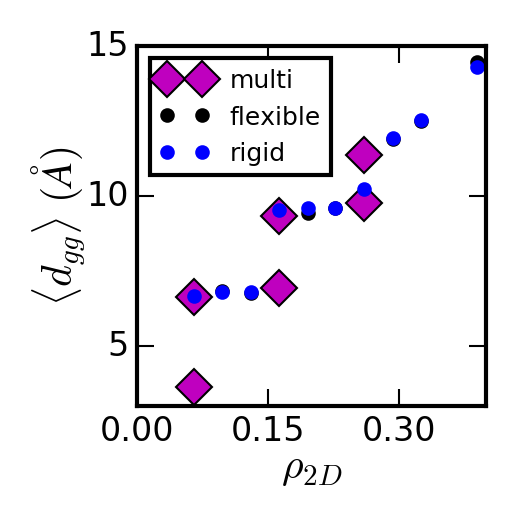
\includegraphics[trim={0.35cm 0.25cm 0.05cm 0.05cm},clip,width=.39\textwidth]{d_gg}
%%		\end{subfigure}
%		\caption{\textit{Plot of average graphene-graphene separation as a function of 2D-number density.} Multi refers to the instances in the flexible case where coexistence between multiple numbers of water layers was observed.}
%		\label{fig:dgg_1}
%	\ang_3B_end{figure}
	
	%%%%%%%%%%%%%%%%%%%%%%%%%%%%%%%%%%%%%%%%
	%%%%%%%%%%%%%%%%%%%%%%%%%%%%%%%%%%%%%%%%

\begin{figure}[h!]
	\centering
	\textbf{6A separation} \\
	\includegraphics[trim={0.99cm 0.25cm 0.25cm 0.15cm},clip,width=0.19\linewidth]{ang_3B_6_0_b} 
	\includegraphics[trim={0.99cm 0.25cm 0.25cm 0.15cm},clip,width=0.19\linewidth]{ang_3B_6_1_b}
	\includegraphics[trim={0.99cm 0.25cm 0.25cm 0.15cm},clip,width=0.19\linewidth]{ang_3B_6_4_b}
	\includegraphics[trim={0.99cm 0.25cm 0.25cm 0.15cm},clip,width=0.19\linewidth]{ang_3B_6_9_b}
	\includegraphics[trim={0.99cm 0.25cm 0.25cm 0.15cm},clip,width=0.19\linewidth]{ang_3B_6_16_b}
	\textbf{8A separation} \\
	\includegraphics[trim={0.99cm 0.25cm 0.25cm 0.15cm},clip,width=0.19\linewidth]{ang_3B_8_0_b} 
	\includegraphics[trim={0.99cm 0.25cm 0.25cm 0.15cm},clip,width=0.19\linewidth]{ang_3B_8_1_b}
	\includegraphics[trim={0.99cm 0.25cm 0.25cm 0.15cm},clip,width=0.19\linewidth]{ang_3B_8_4_b}
	\includegraphics[trim={0.99cm 0.25cm 0.25cm 0.15cm},clip,width=0.19\linewidth]{ang_3B_8_9_b}
	\includegraphics[trim={0.99cm 0.25cm 0.25cm 0.15cm},clip,width=0.19\linewidth]{ang_3B_8_16_b}
	\textbf{9A separation} \\
	\includegraphics[trim={0.99cm 0.25cm 0.25cm 0.15cm},clip,width=0.19\linewidth]{ang_3B_9_0_b} 
	\includegraphics[trim={0.99cm 0.25cm 0.25cm 0.15cm},clip,width=0.19\linewidth]{ang_3B_9_1_b}
	\includegraphics[trim={0.99cm 0.25cm 0.25cm 0.15cm},clip,width=0.19\linewidth]{ang_3B_9_4_b}
	\includegraphics[trim={0.99cm 0.25cm 0.25cm 0.15cm},clip,width=0.19\linewidth]{ang_3B_9_9_b}
	\includegraphics[trim={0.99cm 0.25cm 0.25cm 0.15cm},clip,width=0.19\linewidth]{ang_3B_9_16_b}
	\textbf{11A separation} \\
	\includegraphics[trim={0.99cm 0.25cm 0.25cm 0.15cm},clip,width=0.19\linewidth]{ang_3B_11_0_b} 
	\includegraphics[trim={0.99cm 0.25cm 0.25cm 0.15cm},clip,width=0.19\linewidth]{ang_3B_11_1_b}
	\includegraphics[trim={0.99cm 0.25cm 0.25cm 0.15cm},clip,width=0.19\linewidth]{ang_3B_11_4_b}
	\includegraphics[trim={0.99cm 0.25cm 0.25cm 0.15cm},clip,width=0.19\linewidth]{ang_3B_11_9_b}
	\includegraphics[trim={0.99cm 0.25cm 0.25cm 0.15cm},clip,width=0.19\linewidth]{ang_3B_11_16_b}
	\textbf{14A separation} \\
	\includegraphics[trim={0.99cm 0.25cm 0.25cm 0.15cm},clip,width=0.19\linewidth]{ang_3B_14_0_b} 
	\includegraphics[trim={0.99cm 0.25cm 0.25cm 0.15cm},clip,width=0.19\linewidth]{ang_3B_14_1_b}
	\includegraphics[trim={0.99cm 0.25cm 0.25cm 0.15cm},clip,width=0.19\linewidth]{ang_3B_14_4_b}
	\includegraphics[trim={0.99cm 0.25cm 0.25cm 0.15cm},clip,width=0.19\linewidth]{ang_3B_14_9_b}
	\includegraphics[trim={0.99cm 0.25cm 0.25cm 0.15cm},clip,width=0.19\linewidth]{ang_3B_14_16_b}
	%\caption{\textit{Oxygen-oxygen radial distribution functions} Two-dimensional radial distribution functions in the plane parallel to the graphene plates (a,f) \(\rho_{2D}\) = 0.065, (b,g) \(\rho_{2D}\) = 0.16, (c,h) \(\rho_{2D}\) = 0.26, (d,i) \(\rho_{2D}\) = 0.33.}
	\label{fig:ang}
\end{figure}

\begin{figure}[h!]
	\centering
	\textbf{6A separation} \\
	\includegraphics[trim={0.99cm 0.25cm 0.75cm 0.15cm},clip,width=0.19\linewidth]{dgg_v_x_6_0_b} 
	\includegraphics[trim={0.99cm 0.25cm 0.75cm 0.15cm},clip,width=0.19\linewidth]{dgg_v_x_6_1_b}
	\includegraphics[trim={0.99cm 0.25cm 0.75cm 0.15cm},clip,width=0.19\linewidth]{dgg_v_x_6_4_b}
	\includegraphics[trim={0.99cm 0.25cm 0.75cm 0.15cm},clip,width=0.19\linewidth]{dgg_v_x_6_9_b}
	\includegraphics[trim={0.99cm 0.25cm 0.75cm 0.15cm},clip,width=0.19\linewidth]{dgg_v_x_6_16_b}
	\textbf{8A separation} \\
	\includegraphics[trim={0.99cm 0.25cm 0.75cm 0.15cm},clip,width=0.19\linewidth]{dgg_v_x_8_0_b} 
	\includegraphics[trim={0.99cm 0.25cm 0.75cm 0.15cm},clip,width=0.19\linewidth]{dgg_v_x_8_1_b}
	\includegraphics[trim={0.99cm 0.25cm 0.75cm 0.15cm},clip,width=0.19\linewidth]{dgg_v_x_8_4_b}
	\includegraphics[trim={0.99cm 0.25cm 0.75cm 0.15cm},clip,width=0.19\linewidth]{dgg_v_x_8_9_b}
	\includegraphics[trim={0.99cm 0.25cm 0.75cm 0.15cm},clip,width=0.19\linewidth]{dgg_v_x_8_16_b}
	\textbf{9A separation} \\
	\includegraphics[trim={0.99cm 0.25cm 0.75cm 0.15cm},clip,width=0.19\linewidth]{dgg_v_x_9_0_b} 
	\includegraphics[trim={0.99cm 0.25cm 0.75cm 0.15cm},clip,width=0.19\linewidth]{dgg_v_x_9_1_b}
	\includegraphics[trim={0.99cm 0.25cm 0.75cm 0.15cm},clip,width=0.19\linewidth]{dgg_v_x_9_4_b}
	\includegraphics[trim={0.99cm 0.25cm 0.75cm 0.15cm},clip,width=0.19\linewidth]{dgg_v_x_9_9_b}
	\includegraphics[trim={0.99cm 0.25cm 0.75cm 0.15cm},clip,width=0.19\linewidth]{dgg_v_x_9_16_b}
	\textbf{11A separation} \\
	\includegraphics[trim={0.99cm 0.25cm 0.75cm 0.15cm},clip,width=0.19\linewidth]{dgg_v_x_11_0_b} 
	\includegraphics[trim={0.99cm 0.25cm 0.75cm 0.15cm},clip,width=0.19\linewidth]{dgg_v_x_11_1_b}
	\includegraphics[trim={0.99cm 0.25cm 0.75cm 0.15cm},clip,width=0.19\linewidth]{dgg_v_x_11_4_b}
	\includegraphics[trim={0.99cm 0.25cm 0.75cm 0.15cm},clip,width=0.19\linewidth]{dgg_v_x_11_9_b}
	\includegraphics[trim={0.99cm 0.25cm 0.75cm 0.15cm},clip,width=0.19\linewidth]{dgg_v_x_11_16_b}
	\textbf{14A separation} \\
	\includegraphics[trim={0.99cm 0.25cm 0.75cm 0.15cm},clip,width=0.19\linewidth]{dgg_v_x_14_0_b} 
	\includegraphics[trim={0.99cm 0.25cm 0.75cm 0.15cm},clip,width=0.19\linewidth]{dgg_v_x_14_1_b}
	\includegraphics[trim={0.99cm 0.25cm 0.75cm 0.15cm},clip,width=0.19\linewidth]{dgg_v_x_14_4_b}
	\includegraphics[trim={0.99cm 0.25cm 0.75cm 0.15cm},clip,width=0.19\linewidth]{dgg_v_x_14_9_b}
	\includegraphics[trim={0.99cm 0.25cm 0.75cm 0.15cm},clip,width=0.19\linewidth]{dgg_v_x_14_16_b}
	%\caption{\textit{Oxygen-oxygen radial distribution functions} Two-dimensional radial distribution functions in the plane parallel to the graphene plates (a,f) \(\rho_{2D}\) = 0.065, (b,g) \(\rho_{2D}\) = 0.16, (c,h) \(\rho_{2D}\) = 0.26, (d,i) \(\rho_{2D}\) = 0.33.}
	\label{fig:ang}
\end{figure}


\begin{figure}[h!]
	\centering
	\textbf{6A separation} \\
	\includegraphics[trim={0.49cm 0.25cm 0.25cm 0.25cm},clip,width=0.19\linewidth]{sol_ang_6_1_b}
	\includegraphics[trim={0.49cm 0.25cm 0.25cm 0.25cm},clip,width=0.19\linewidth]{sol_ang_6_4_b}
	\includegraphics[trim={0.49cm 0.25cm 0.25cm 0.25cm},clip,width=0.19\linewidth]{sol_ang_6_9_b}
	\includegraphics[trim={0.49cm 0.25cm 0.25cm 0.25cm},clip,width=0.19\linewidth]{sol_ang_6_16_b}
	\\ \textbf{8A separation} \\
	\includegraphics[trim={0.49cm 0.25cm 0.25cm 0.25cm},clip,width=0.19\linewidth]{sol_ang_8_1_b}
	\includegraphics[trim={0.49cm 0.25cm 0.25cm 0.25cm},clip,width=0.19\linewidth]{sol_ang_8_4_b}
	\includegraphics[trim={0.49cm 0.25cm 0.25cm 0.25cm},clip,width=0.19\linewidth]{sol_ang_8_9_b}
	\includegraphics[trim={0.49cm 0.25cm 0.25cm 0.25cm},clip,width=0.19\linewidth]{sol_ang_8_16_b}
	\\ \textbf{9A separation} \\
	\includegraphics[trim={0.49cm 0.25cm 0.25cm 0.25cm},clip,width=0.19\linewidth]{sol_ang_9_1_b}
	\includegraphics[trim={0.49cm 0.25cm 0.25cm 0.25cm},clip,width=0.19\linewidth]{sol_ang_9_4_b}
	\includegraphics[trim={0.49cm 0.25cm 0.25cm 0.25cm},clip,width=0.19\linewidth]{sol_ang_9_9_b}
	\includegraphics[trim={0.49cm 0.25cm 0.25cm 0.25cm},clip,width=0.19\linewidth]{sol_ang_9_16_b}
	\\ \textbf{11A separation} \\
	\includegraphics[trim={0.49cm 0.25cm 0.25cm 0.25cm},clip,width=0.19\linewidth]{sol_ang_11_1_b}
	\includegraphics[trim={0.49cm 0.25cm 0.25cm 0.25cm},clip,width=0.19\linewidth]{sol_ang_11_4_b}
	\includegraphics[trim={0.49cm 0.25cm 0.25cm 0.25cm},clip,width=0.19\linewidth]{sol_ang_11_9_b}
	\includegraphics[trim={0.49cm 0.25cm 0.25cm 0.25cm},clip,width=0.19\linewidth]{sol_ang_11_16_b}
	\\ \textbf{14A separation} \\
	\includegraphics[trim={0.49cm 0.25cm 0.25cm 0.25cm},clip,width=0.19\linewidth]{sol_ang_14_1_b}
	\includegraphics[trim={0.49cm 0.25cm 0.25cm 0.25cm},clip,width=0.19\linewidth]{sol_ang_14_4_b}
	\includegraphics[trim={0.49cm 0.25cm 0.25cm 0.25cm},clip,width=0.19\linewidth]{sol_ang_14_9_b}
	\includegraphics[trim={0.49cm 0.25cm 0.25cm 0.25cm},clip,width=0.19\linewidth]{sol_ang_14_16_b}
	%\caption{\textit{Oxygen-oxygen radial distribution functions} Two-dimensional radial distribution functions in the plane parallel to the graphene plates (a,f) \(\rho_{2D}\) = 0.065, (b,g) \(\rho_{2D}\) = 0.16, (c,h) \(\rho_{2D}\) = 0.26, (d,i) \(\rho_{2D}\) = 0.33.}
	\label{fig:ang_sol}
\end{figure}

%\begin{figure}[h!]
%	\centering
%	\textbf{6A separation} \\
%	\includegraphics[trim={0.49cm 0.25cm 0.25cm 0.25cm},clip,width=0.19\linewidth]{sol_dist_6_1_b}
%	\includegraphics[trim={0.49cm 0.25cm 0.25cm 0.25cm},clip,width=0.19\linewidth]{sol_dist_6_4_b}
%	\includegraphics[trim={0.49cm 0.25cm 0.25cm 0.25cm},clip,width=0.19\linewidth]{sol_dist_6_9_b}
%	\includegraphics[trim={0.49cm 0.25cm 0.25cm 0.25cm},clip,width=0.19\linewidth]{sol_dist_6_16_b}
%	\\ \textbf{8A separation} \\
%	\includegraphics[trim={0.49cm 0.25cm 0.25cm 0.25cm},clip,width=0.19\linewidth]{sol_dist_8_1_b}
%	\includegraphics[trim={0.49cm 0.25cm 0.25cm 0.25cm},clip,width=0.19\linewidth]{sol_dist_8_4_b}
%	\includegraphics[trim={0.49cm 0.25cm 0.25cm 0.25cm},clip,width=0.19\linewidth]{sol_dist_8_9_b}
%	\includegraphics[trim={0.49cm 0.25cm 0.25cm 0.25cm},clip,width=0.19\linewidth]{sol_dist_8_16_b}
%	\\ \textbf{9A separation} \\
%	\includegraphics[trim={0.49cm 0.25cm 0.25cm 0.25cm},clip,width=0.19\linewidth]{sol_dist_9_1_b}
%	\includegraphics[trim={0.49cm 0.25cm 0.25cm 0.25cm},clip,width=0.19\linewidth]{sol_dist_9_4_b}
%	\includegraphics[trim={0.49cm 0.25cm 0.25cm 0.25cm},clip,width=0.19\linewidth]{sol_dist_9_9_b}
%	\includegraphics[trim={0.49cm 0.25cm 0.25cm 0.25cm},clip,width=0.19\linewidth]{sol_dist_9_16_b}
%	\\ \textbf{11A separation} \\
%	\includegraphics[trim={0.49cm 0.25cm 0.25cm 0.25cm},clip,width=0.19\linewidth]{sol_dist_11_1_b}
%	\includegraphics[trim={0.49cm 0.25cm 0.25cm 0.25cm},clip,width=0.19\linewidth]{sol_dist_11_4_b}
%	\includegraphics[trim={0.49cm 0.25cm 0.25cm 0.25cm},clip,width=0.19\linewidth]{sol_dist_11_9_b}
%	\includegraphics[trim={0.49cm 0.25cm 0.25cm 0.25cm},clip,width=0.19\linewidth]{sol_dist_11_16_b}
%	\\ \textbf{14A separation} \\
%	\includegraphics[trim={0.49cm 0.25cm 0.25cm 0.25cm},clip,width=0.19\linewidth]{sol_dist_14_1_b}
%	\includegraphics[trim={0.49cm 0.25cm 0.25cm 0.25cm},clip,width=0.19\linewidth]{sol_dist_14_4_b}
%	\includegraphics[trim={0.49cm 0.25cm 0.25cm 0.25cm},clip,width=0.19\linewidth]{sol_dist_14_9_b}
%	\includegraphics[trim={0.49cm 0.25cm 0.25cm 0.25cm},clip,width=0.19\linewidth]{sol_dist_14_16_b}
%	%\caption{\textit{Oxygen-oxygen radial distribution functions} Two-dimensional radial distribution functions in the plane parallel to the graphene plates (a,f) \(\rho_{2D}\) = 0.065, (b,g) \(\rho_{2D}\) = 0.16, (c,h) \(\rho_{2D}\) = 0.26, (d,i) \(\rho_{2D}\) = 0.33.}
%	\label{fig:dist_sol}
%\end{figure}

\begin{figure}[h!]
	\centering
	\textbf{6A separation} \\
	\includegraphics[trim={0.49cm 0.25cm 0.25cm 0.25cm},clip,width=0.19\linewidth]{sol_neigh_6_1_b}
	\includegraphics[trim={0.49cm 0.25cm 0.25cm 0.25cm},clip,width=0.19\linewidth]{sol_neigh_6_4_b}
	\includegraphics[trim={0.49cm 0.25cm 0.25cm 0.25cm},clip,width=0.19\linewidth]{sol_neigh_6_9_b}
	\includegraphics[trim={0.49cm 0.25cm 0.25cm 0.25cm},clip,width=0.19\linewidth]{sol_neigh_6_16_b}
	\\ \textbf{8A separation} \\
	\includegraphics[trim={0.49cm 0.25cm 0.25cm 0.25cm},clip,width=0.19\linewidth]{sol_neigh_8_1_b}
	\includegraphics[trim={0.49cm 0.25cm 0.25cm 0.25cm},clip,width=0.19\linewidth]{sol_neigh_8_4_b}
	\includegraphics[trim={0.49cm 0.25cm 0.25cm 0.25cm},clip,width=0.19\linewidth]{sol_neigh_8_9_b}
	\includegraphics[trim={0.49cm 0.25cm 0.25cm 0.25cm},clip,width=0.19\linewidth]{sol_neigh_8_16_b}
	\\ \textbf{9A separation} \\
	\includegraphics[trim={0.49cm 0.25cm 0.25cm 0.25cm},clip,width=0.19\linewidth]{sol_neigh_9_1_b}
	\includegraphics[trim={0.49cm 0.25cm 0.25cm 0.25cm},clip,width=0.19\linewidth]{sol_neigh_9_4_b}
	\includegraphics[trim={0.49cm 0.25cm 0.25cm 0.25cm},clip,width=0.19\linewidth]{sol_neigh_9_9_b}
	\includegraphics[trim={0.49cm 0.25cm 0.25cm 0.25cm},clip,width=0.19\linewidth]{sol_neigh_9_16_b}
	\\ \textbf{11A separation} \\
	\includegraphics[trim={0.49cm 0.25cm 0.25cm 0.25cm},clip,width=0.19\linewidth]{sol_neigh_11_1_b}
	\includegraphics[trim={0.49cm 0.25cm 0.25cm 0.25cm},clip,width=0.19\linewidth]{sol_neigh_11_4_b}
	\includegraphics[trim={0.49cm 0.25cm 0.25cm 0.25cm},clip,width=0.19\linewidth]{sol_neigh_11_9_b}
	\includegraphics[trim={0.49cm 0.25cm 0.25cm 0.25cm},clip,width=0.19\linewidth]{sol_neigh_11_16_b}
	\\ \textbf{14A separation} \\
	\includegraphics[trim={0.49cm 0.25cm 0.25cm 0.25cm},clip,width=0.19\linewidth]{sol_neigh_14_1_b}
	\includegraphics[trim={0.49cm 0.25cm 0.25cm 0.25cm},clip,width=0.19\linewidth]{sol_neigh_14_4_b}
	\includegraphics[trim={0.49cm 0.25cm 0.25cm 0.25cm},clip,width=0.19\linewidth]{sol_neigh_14_9_b}
	\includegraphics[trim={0.49cm 0.25cm 0.25cm 0.25cm},clip,width=0.19\linewidth]{sol_neigh_14_16_b}
	%\caption{\textit{Oxygen-oxygen radial distribution functions} Two-dimensional radial distribution functions in the plane parallel to the graphene plates (a,f) \(\rho_{2D}\) = 0.065, (b,g) \(\rho_{2D}\) = 0.16, (c,h) \(\rho_{2D}\) = 0.26, (d,i) \(\rho_{2D}\) = 0.33.}
	\label{fig:neigh_sol}
\end{figure}

\begin{figure}[h!]
	\centering
	\textbf{9A separation} \\
	\includegraphics[trim={0.39cm 0.25cm 0.25cm 0.15cm},clip,width=0.19\linewidth]{g_r_9_5_b_o_o} 
	\includegraphics[trim={0.39cm 0.25cm 0.25cm 0.15cm},clip,width=0.19\linewidth]{g_r_9_6_b_o_o}
	\includegraphics[trim={0.39cm 0.25cm 0.25cm 0.15cm},clip,width=0.19\linewidth]{g_r_9_7_b_o_o}
	\includegraphics[trim={0.39cm 0.25cm 0.25cm 0.15cm},clip,width=0.19\linewidth]{g_r_9_8_b_o_o}
	\includegraphics[trim={0.39cm 0.25cm 0.25cm 0.15cm},clip,width=0.19\linewidth]{g_r_9_24_b_o_o}
	\textbf{9A separation} \\
	\includegraphics[trim={0.99cm 0.25cm 0.25cm 0.15cm},clip,width=0.19\linewidth]{ang_3B_9_5_b} 
	\includegraphics[trim={0.99cm 0.25cm 0.25cm 0.15cm},clip,width=0.19\linewidth]{ang_3B_9_6_b}
	\includegraphics[trim={0.99cm 0.25cm 0.25cm 0.15cm},clip,width=0.19\linewidth]{ang_3B_9_7_b}
	\includegraphics[trim={0.99cm 0.25cm 0.25cm 0.15cm},clip,width=0.19\linewidth]{ang_3B_9_8_b}
	\includegraphics[trim={0.99cm 0.25cm 0.25cm 0.15cm},clip,width=0.19\linewidth]{ang_3B_9_24_b}
	\textbf{9A separation} \\
	\includegraphics[trim={0.49cm 0.25cm 0.25cm 0.15cm},clip,width=0.19\linewidth]{sol_ang_9_5_b} 
	\includegraphics[trim={0.49cm 0.25cm 0.25cm 0.15cm},clip,width=0.19\linewidth]{sol_ang_9_6_b}
	\includegraphics[trim={0.49cm 0.25cm 0.25cm 0.15cm},clip,width=0.19\linewidth]{sol_ang_9_7_b}
	\includegraphics[trim={0.49cm 0.25cm 0.25cm 0.15cm},clip,width=0.19\linewidth]{sol_ang_9_8_b}
	\includegraphics[trim={0.49cm 0.25cm 0.25cm 0.15cm},clip,width=0.19\linewidth]{sol_ang_9_24_b}
	\textbf{9A separation} \\
	\includegraphics[trim={0.49cm 0.25cm 0.25cm 0.15cm},clip,width=0.19\linewidth]{sol_neigh_9_5_b} 
	\includegraphics[trim={0.49cm 0.25cm 0.25cm 0.15cm},clip,width=0.19\linewidth]{sol_neigh_9_6_b}
	\includegraphics[trim={0.49cm 0.25cm 0.25cm 0.15cm},clip,width=0.19\linewidth]{sol_neigh_9_7_b}
	\includegraphics[trim={0.49cm 0.25cm 0.25cm 0.15cm},clip,width=0.19\linewidth]{sol_neigh_9_8_b}
	\includegraphics[trim={0.49cm 0.25cm 0.25cm 0.15cm},clip,width=0.19\linewidth]{sol_neigh_9_24_b}
	%\caption{\textit{Oxygen-oxygen radial distribution functions} Two-dimensional radial distribution functions in the plane parallel to the graphene plates (a,f) \(\rho_{2D}\) = 0.065, (b,g) \(\rho_{2D}\) = 0.16, (c,h) \(\rho_{2D}\) = 0.26, (d,i) \(\rho_{2D}\) = 0.33.}
	\label{fig:gr_9extra}
\end{figure}


\begin{figure}[h!]
	\centering
	 \includegraphics[width=0.50\linewidth]{lege_dens_w} \\
	 \textbf{\(D_{gg}\)}  \quad \quad \quad  \quad \quad \quad  \quad \quad \quad \textbf{Compressibility} \quad \quad \quad \quad \quad \textbf{Diffusion 2D}   \\
	\includegraphics[trim={0.29cm 0.25cm 0.25cm 0.15cm},clip,width=0.31\linewidth]{d_gg} 
	% \\ \textbf{Compressibility} \\
	\includegraphics[trim={0.29cm 0.25cm 0.25cm 0.15cm},clip,width=0.29\linewidth]{compressibility} 
	% \\ \textbf{Diffusion 2D} \\
	\includegraphics[trim={0.29cm 0.25cm 0.25cm 0.15cm},clip,width=0.30\linewidth]{diffusion} 
	%\caption{\textit{Oxygen-oxygen radial distribution functions} Two-dimensional radial distribution functions in the plane parallel to the graphene plates (a,f) \(\rho_{2D}\) = 0.065, (b,g) \(\rho_{2D}\) = 0.16, (c,h) \(\rho_{2D}\) = 0.26, (d,i) \(\rho_{2D}\) = 0.33.}
	\label{fig:gr_9extra}
\end{figure}

\setlength{\fboxsep}{0.75pt}%
\setlength{\fboxrule}{1.2pt}%

%\begin{figure}[ht!]
%	\centering
%	\includegraphics[width=0.46\textwidth]{leg_bulk_6_7_8}\\
%  \fbox{\begin{subfigure}[b]{0.47\textwidth}
%    \includegraphics[trim={0.05cm 0.30cm 0.25cm 0.15cm},clip,width=0.46\textwidth]{g_r_2D_6_7_8_r}
%    \includegraphics[trim={0.25cm 0.25cm 0.05cm 0.15cm},clip,width=0.485\textwidth]{ang_3B_6_7_8_r} 
%     \fbox{\includegraphics[width=0.29\textwidth]{6A_r0} 
%             	\llap{\raisebox{-0.4cm}{\color{white} \small  \fcolorbox{black}{black}{\(\mathcal{D}_{||}=2.26\)}}}}
%     \fbox{\includegraphics[width=0.29\textwidth]{7A_r0}
%     		\llap{\raisebox{-0.4cm}{\color{white} \small  \fcolorbox{red}{red}{\(\mathcal{D}_{||}=5.4e\scalebox{0.75}[1.0]{\( - \)}3\)}}}}
%     \fbox{\includegraphics[width=0.29\textwidth]{8A_r0}
%     		\llap{\raisebox{-0.4cm}{\color{white} \small  \fcolorbox{blue}{blue}{\(\mathcal{D}_{||}=1.4e\scalebox{0.75}[1.0]{\( - \)}4\)}}}}
%    \caption{}
%    \label{fig:gr_ang_6_7_8_r}
%  \end{subfigure}}
%  \fbox{\begin{subfigure}[b]{0.47\textwidth}
%    \includegraphics[trim={0.05cm 0.30cm 0.25cm 0.15cm},clip,width=0.46\textwidth]{g_r_2D_6_7_8_f}
%    \includegraphics[trim={0.25cm 0.25cm 0.05cm 0.15cm},clip,width=0.485\textwidth]{ang_3B_6_7_8_f}
%     \fbox{\includegraphics[width=0.29\textwidth]{6A_f0}
%     		\llap{\raisebox{-0.4cm}{\color{white} \small \fcolorbox{black}{black}{\(\mathcal{D}_{||}=3.2e\scalebox{0.75}[1.0]{\( - \)}4\)}}}} %\raisebox{1.8cm} for in upper right corner
%     \fbox{\includegraphics[width=0.29\textwidth]{7A_f0}
%     		\llap{\raisebox{-0.4cm}{\color{white} \small \fcolorbox{red}{red}{\(\mathcal{D}_{||}=3.35\)}}}}
%     \fbox{\includegraphics[width=0.29\textwidth]{8A_f0}
%     		\llap{\raisebox{-0.4cm}{\color{white} \small \fcolorbox{blue}{blue}{\(\mathcal{D}_{||}=1.3e\scalebox{0.75}[1.0]{\( - \)}2\)}}}}
%    \caption{}
%    \label{fig:gr_ang_6_7_8_f}
%  \end{subfigure}}
%	\caption{\textit{Monolayer lateral oxygen-oxygen pair correlation functions, three-body angle distributions, and snapshots of monolayer systems.} (\protect\subref{fig:gr_ang_6_7_8_r}) rigid systems, (\protect\subref{fig:gr_ang_6_7_8_f}) flexible systems.  \textbf{Top.} Distribution of water oxygen distances and distribution of intralayer 3B angle formed between and given oxygen and its 2 nearest neighbors. \textbf{Bottom.} Snapshots of systems from left to right: \(\rho_{2D}=\) 0.062, 0.092, 0.123. Oxygens are in red, hydrogens are in white and for clarity, only one interlayer of water is depicted, and the graphene sheets are not displayed. Lateral diffusion coefficients are given in units of \((m^2/s) \times 10^9\), in the colored box in the bottom right corner. The lowest density system of (\protect\subref{fig:gr_ang_6_7_8_f}) is comprised of a coexistence between different number of water interlayers, highlighted in black (n=0) and blue (n=1).}
%	\label{fig:struct_6_7_8}
%\end{figure}

\clearpage
\clearpage
%%%%%%%%%%%%%%%%%%%%%%%%%%%%%%%%%%%%%%%%
%%%%%%%%%%%%%%%%%%%%%%%%%%%%%%%%%%%%%%%%
%%%%%%%%%%%%%%%%%%%%%%%%%%%%%%%%%%%%%%%%
%%%%%%%%%%%%%%%%%%%%%%%%%%%%%%%%%%%%%%%%
\section{Computational Methods}
	
	The model system consists of two parallel graphene sheets with water molecules filling the two interlayer spacings at a prescribed density \(\rho_{2D}\). The confinement occurs in the x-direction, and the in-plane dimensions of the system are \(L_y\) = 46.2 \r A, and  \(L_z\) = 48.5 \r A. Periodic boundary conditions are applied in all dimensions. We use the TIP4P-Ew model of water \cite{Horn2004}, and the parameters for graphene have been adapted from previous works \cite{Hummer2001,Patra2009}. All the bonded parameters are summarized in Table \ref{table:ff_parms}, and the non-bonded parameters in Table \ref{table:ff_parms_atoms}. 
	
	\begin{table}[ht!]
		\caption{\textit{Force field bonded parameters used for graphene in confined water simulations.}}
		\label{table:ff_parms}
		\centering
		\begin{tabular}{  l |  l l l } \hline
			\textbf{bonded term}  &\multicolumn{3}{c}{\textbf{parameters}} \\ \hline
			Bond  & \(K_b\)  (\(kCal/mol/\angstrom^2\))      & b\textsubscript{0}  (\r A)  &  \\ %\hline
			   & 938.0         & 1.40            &    \\   \hline
			Angle & \(K_{\theta}\)  (\(kCal/mol/rad^2\)) & \(\theta_0\) (degrees)   &          \\ 
			  & 126.0         & 120.0           &         \\ \hline
			Improper   & K\textsubscript{im} (kCal/mol)       & \(\chi_0\) (degrees)     &          \\ 
			 & 15.0          & 0.0             &          \\ \hline
			Dihedral      & K\textsubscript{di} (kCal/mol)       & n (multiplicity) & \(\phi\) (degrees)\\ 
			 & 3.150         & 2               & 180.0  \\  \hline
		\end{tabular}
	\end{table}
	
	\begin{table}[ht!]
		\caption{Force field parameters used for each atom type in confined water simulations.}
		\label{table:ff_parms_atoms}
		\begin{tabular}{ c|r|r|r}
			\hline
			\textbf{atom type} & \multicolumn{1}{c|}{\textbf{\begin{tabular}[c]{@{}c@{}}partial charge\\ (e)\end{tabular}}} & \multicolumn{1}{c|}{\textbf{\begin{tabular}[c]{@{}c@{}}\(\sigma\)\\ (\r A)\end{tabular}}} & \multicolumn{1}{c}{\textbf{\begin{tabular}[c]{@{}c@{}}\(\epsilon\)\\ (kCal/mole)\end{tabular}}} \\ \hline
			Graphene carbon & 0.0000  & 3.55 & 0.07   \\ 
			Water oxygen       & -1.0484 & 3.16435  & 0.16275  \\ 
			Water hydrogen   & 0.5242  & 0.00000 & 0.00000  \\ \hline
		\end{tabular}
	\end{table}

	All the simulations were performed with the LAMMPS software package \cite{Plimpton1995}. We use a time step of 2.0 fs for all the simulations, and all the simulations are performed at T = 298 K. We use the SHAKE algorithm \cite{Andersen1983} with a tolerance of 10\textsuperscript{-4} to keep the water molecules rigid, according to the TIP4P-Ew water model \cite{Horn2004}. Initially, we relax the system at constant volume in two steps. First, to get rid of close contacts or other high-energy configurations in the system, we run Brownian dynamics \cite{Schneider1978} for a short 10 ps where we limit the atoms displacement in a single time step to 0.1 \r A. After that, we simulate the system in the NVT ensemble for another 10 ps using a temperature damping parameter of 0.1 ps. After relaxing the system at constant volume, we perform runs of 10 ns in the NpT ensemble, where only the x-direction (i.e. the direction of confinement) is allowed to fluctuate, \(p_{xx}\) = 0.1 MPa. The temperature and pressure control were implemented using a Nos\' e-Hoover extended Lagrangian procedure \cite{Martyna1994} with characteristic damping times 0.1 and 1.0 ps, respectively. We consider the first 3 ns equilibration, and we collect data for analysis every 500 steps (2 ps) over the last 7 ns of the NpT trajectories. In the rigid cases, the graphene sheets are kept rigid but their center of mass position can fluctuate. In the flexible cases the full force-field is employed without further constraints.


%%%%%%%%%%%%%%%%%%%%%%%%%%%%%%%%%%%%%%%%%%%%%%%%%%%%%%%%%%%%%%%%%%%%%
%% The "Acknowledgement" section can be given in all manuscript
%% classes.  This should be given within the "acknowledgement"
%% environment, which will make the correct section or running title.
%%%%%%%%%%%%%%%%%%%%%%%%%%%%%%%%%%%%%%%%%%%%%%%%%%%%%%%%%%%%%%%%%%%%%
\begin{acknowledgement}

Please use ``The authors thank \ldots'' rather than ``The
authors would like to thank \ldots''.

\end{acknowledgement}

%%%%%%%%%%%%%%%%%%%%%%%%%%%%%%%%%%%%%%%%%%%%%%%%%%%%%%%%%%%%%%%%%%%%%
%% The same is true for Supporting Information, which should use the
%% suppinfo environment.
%%%%%%%%%%%%%%%%%%%%%%%%%%%%%%%%%%%%%%%%%%%%%%%%%%%%%%%%%%%%%%%%%%%%%
\begin{suppinfo}

A listing of the contents of each file supplied as Supporting Information
should be included. For instructions on what should be included in the
Supporting Information as well as how to prepare this material for
publications, refer to the journal's Instructions for Authors.

The following files are available free of charge.
\begin{itemize}
  \item Filename: brief description
  \item Filename: brief description
\end{itemize}

\end{suppinfo}

%%%%%%%%%%%%%%%%%%%%%%%%%%%%%%%%%%%%%%%%%%%%%%%%%%%%%%%%%%%%%%%%%%%%%
%% The appropriate \bibliography command should be placed here.
%% Notice that the class file automatically sets \bibliographystyle
%% and also names the section correctly.
%%%%%%%%%%%%%%%%%%%%%%%%%%%%%%%%%%%%%%%%%%%%%%%%%%%%%%%%%%%%%%%%%%%%%
\bibliography{references}

\end{document}
